\subsection{Cellular Networks}\label{subsec:Cell_Networks}
Cellular networks are setup in the \nameref{subsubsec:Licensed_Spectrum}s.
They are the major backbone of data infrastructure that is not completely tied to a physical location.

\subsubsection{GSM (2G)}\label{subsubsec:2G}
To reuse the frequencies in GSM, we can subdivide an area into cells.
These cells are idealized to hexagons, and each hexagon gets its own frequency.
Then, any hexagons in adjacent zones cannot have the same frequencies near its border.

The repeating distance of these cells is given in \Cref{eq:GSM_Cell_Repeat_Distance}.
\begin{equation}\label{eq:GSM_Cell_Repeat_Distance}
  D = R \sqrt{3K}
\end{equation}
\begin{itemize}[noitemsep]
\item $R$: Cell radius (How large are the hexagons?)
\item $K$: Cluster size (How many hexagons are allowed?)
\item $D$: The repeating distance (How far between hexagons that repeat the same frequency?)
\end{itemize}

\subsubsection{UMTS (3G)}\label{subsubsec:3G}
Used \nameref{def:CDMA}

\subsubsection{LTE (4G)}\label{subsubsec:4G}
\begin{definition}[LTE]\label{def:LTE}
  \emph{LTE} or \emph{Long Term Evolution} is a standard that was finalized in 2008, and first publicaly available in 2009.
  Its main goals were to increase speed and capacity, while using a simpler IP-based network architecture.
  This was dirven by the large increase in data usage compared to phone calls made.

  The LTE radio interface was incompatible with previous 2G and 3G networks.

  The biggest feature was the concept of \textbf{\nameref{def:Bearer}s}.
  This allows for different Quality of Services for different classes of network traffic.
\end{definition}

\paragraph{Bearers}\label{par:Bearers}
\begin{definition}[Bearer]\label{def:Bearer}
  \emph{Bearer}s are a way to ensure Quality of Service.

  \begin{itemize}[noitemsep]
  \item Minimum Guaranteed Bitrate (GBR)
    \begin{itemize}[noitemsep]
    \item Dedicated resources permanently allocated at bearer establishment
    \item Higher bitrates may be allowed when resources are available
    \end{itemize}

  \item Non-GBR, e.g. FTP, web browsing
    \begin{itemize}[noitemsep]
    \item Best effort service
    \item No resources allocated
    \item QoS class identifier (QCI): priority, packet delay budget, acceptable packet loss rate
    \end{itemize}
  \end{itemize}
\end{definition}

\subsubsection{5G}\label{subsubsec:5G}
\begin{definition}[5G]\label{def:5G}
  \emph{5G} is the next generation of wireless cellular communications.
  It offers many improvements over 4G LTE and will be used nearly everywhere in the digital world.
\end{definition}

\begin{remark*}
  There are a lot of abbreviations in the comming sections.
  I apologize for this, but I have no say in the matter.
  I am including them to make sure there is a good reference for many of these.
\end{remark*}

\paragraph{Software Defined Networking}\label{par:SDN}
\begin{definition}[Software Defined Networking]\label{def:Software_Defined_Networking}

\end{definition}
\textbf{TODO!!}
\begin{figure}[h!tbp]
  \centering
  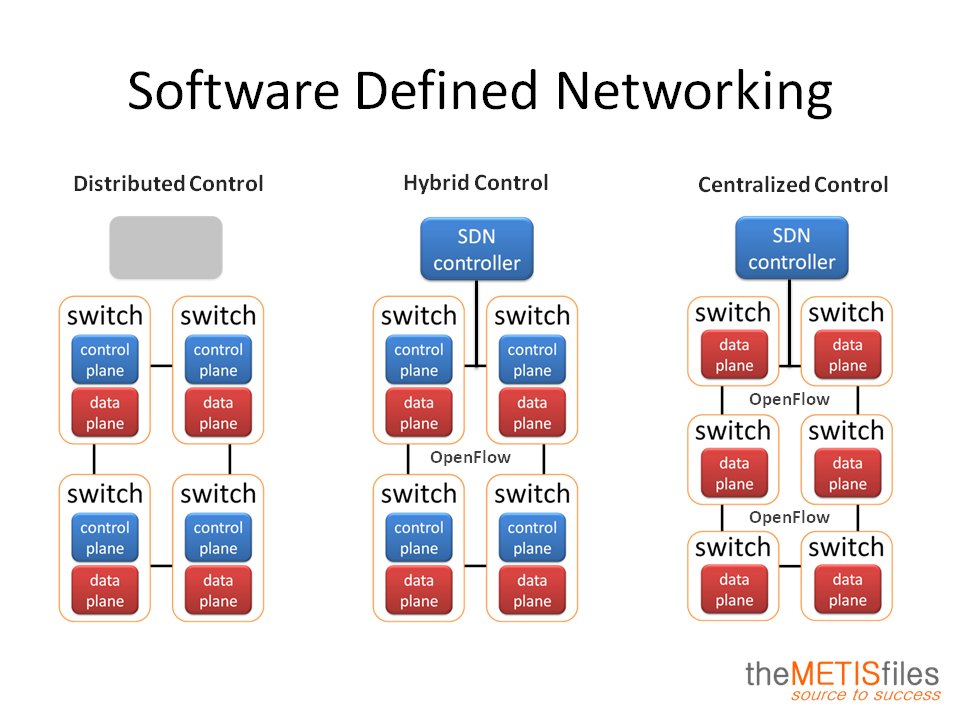
\includegraphics[scale=0.5]{./Drawings/ETSN10-Network_Architecture_Performance/software-defined-networking.png}
  \caption{Software Defined Networking\footnote{\url{https://www.themetisfiles.com/2012/10/the-future-of-the-network-is-software-defined/}}}
  \label{fig:SDN}
\end{figure}

\paragraph{Network Function Virtualization}\label{par:NFV}
\textbf{TODO!!}

\paragraph{Network Slicing}\label{par:Network_Slicing}
\begin{definition}[Network Slicing]\label{def:Network_Slicing}

\end{definition}
\textbf{TODO!!}

\paragraph{Cloud RAN}\label{par:Cloud_RAN}
\begin{definition}[Cloud Radio Access Network]\label{def:Cloud_RAN}

\end{definition}
\textbf{TODO!!}

\paragraph{Frame Structure}\label{par:Frame_Structure}
\textbf{TODO!!}

\paragraph{Enabling Technologies for 5G}\label{par:5G_Enabling_Technologies}
\textbf{TODO!!}

\subparagraph{Millimeter Wave}\label{subpar:Millimeter_Wave}
\textbf{TODO!!}

\subparagraph{Small Cells}\label{subpar:Small_Cells}
\textbf{TODO!!}

\subparagraph{Massive MIMO}\label{subpar:Massive_MIMO}
\textbf{TODO!!}

%%% Local Variables:
%%% mode: latex
%%% TeX-master: "../../ETSN10-Network_Architecture_Performance-Reference_Sheet"
%%% End:
